\subsection{Who is Immigrant}\label{sec:immig}

\subsection{Age Profile of Public Tranfer}\label{sec:profile}

\autoref{fig:txAge9715} show the age profiles of cost-contribution for 1997 and 2015 as examples. Compatible with the life cycle theories of consumption, cost-contributions are positive at younger and older ages but negative during prime age as production surpasses consumption.

\begin{figure}[H]%
  \caption{ Cost-contribution profile for Native and Immmigrants for 1997 and 2015}
  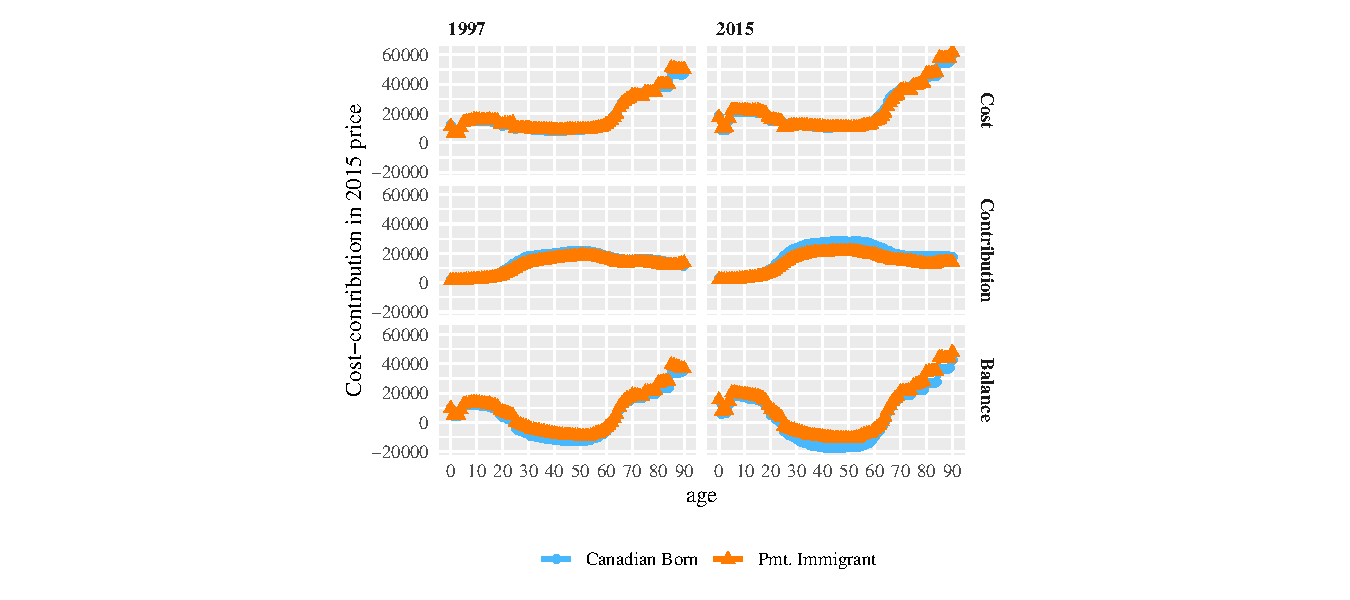
\includegraphics[width=1\textwidth]{./res/txAge9715.pdf}%
  \label{fig:txAge9715}%
\end{figure}%




To account for the difference in age structure by immigration status, we standardize the age profiles with the age structure of the 2011 population census. Results are quite differentes from previous ones.

For instance, the difference in net transfer between native on one hand and  immigrant group on the other hand has increased to ()



This leads to an increase in net contributions of 660\$ for a native and net costs of about 2930\$ for an immigrant

\autoref{fig:txSumAj} and \autoref{fig:txTrendAj} present the age Ajusted summaries and trend using the population structure from the 2011 population census
  \begin{figure}[H]%
    \caption{Age Ajusted Cost Contribution Summaries by Immigration Status between 1997 and 2015}
    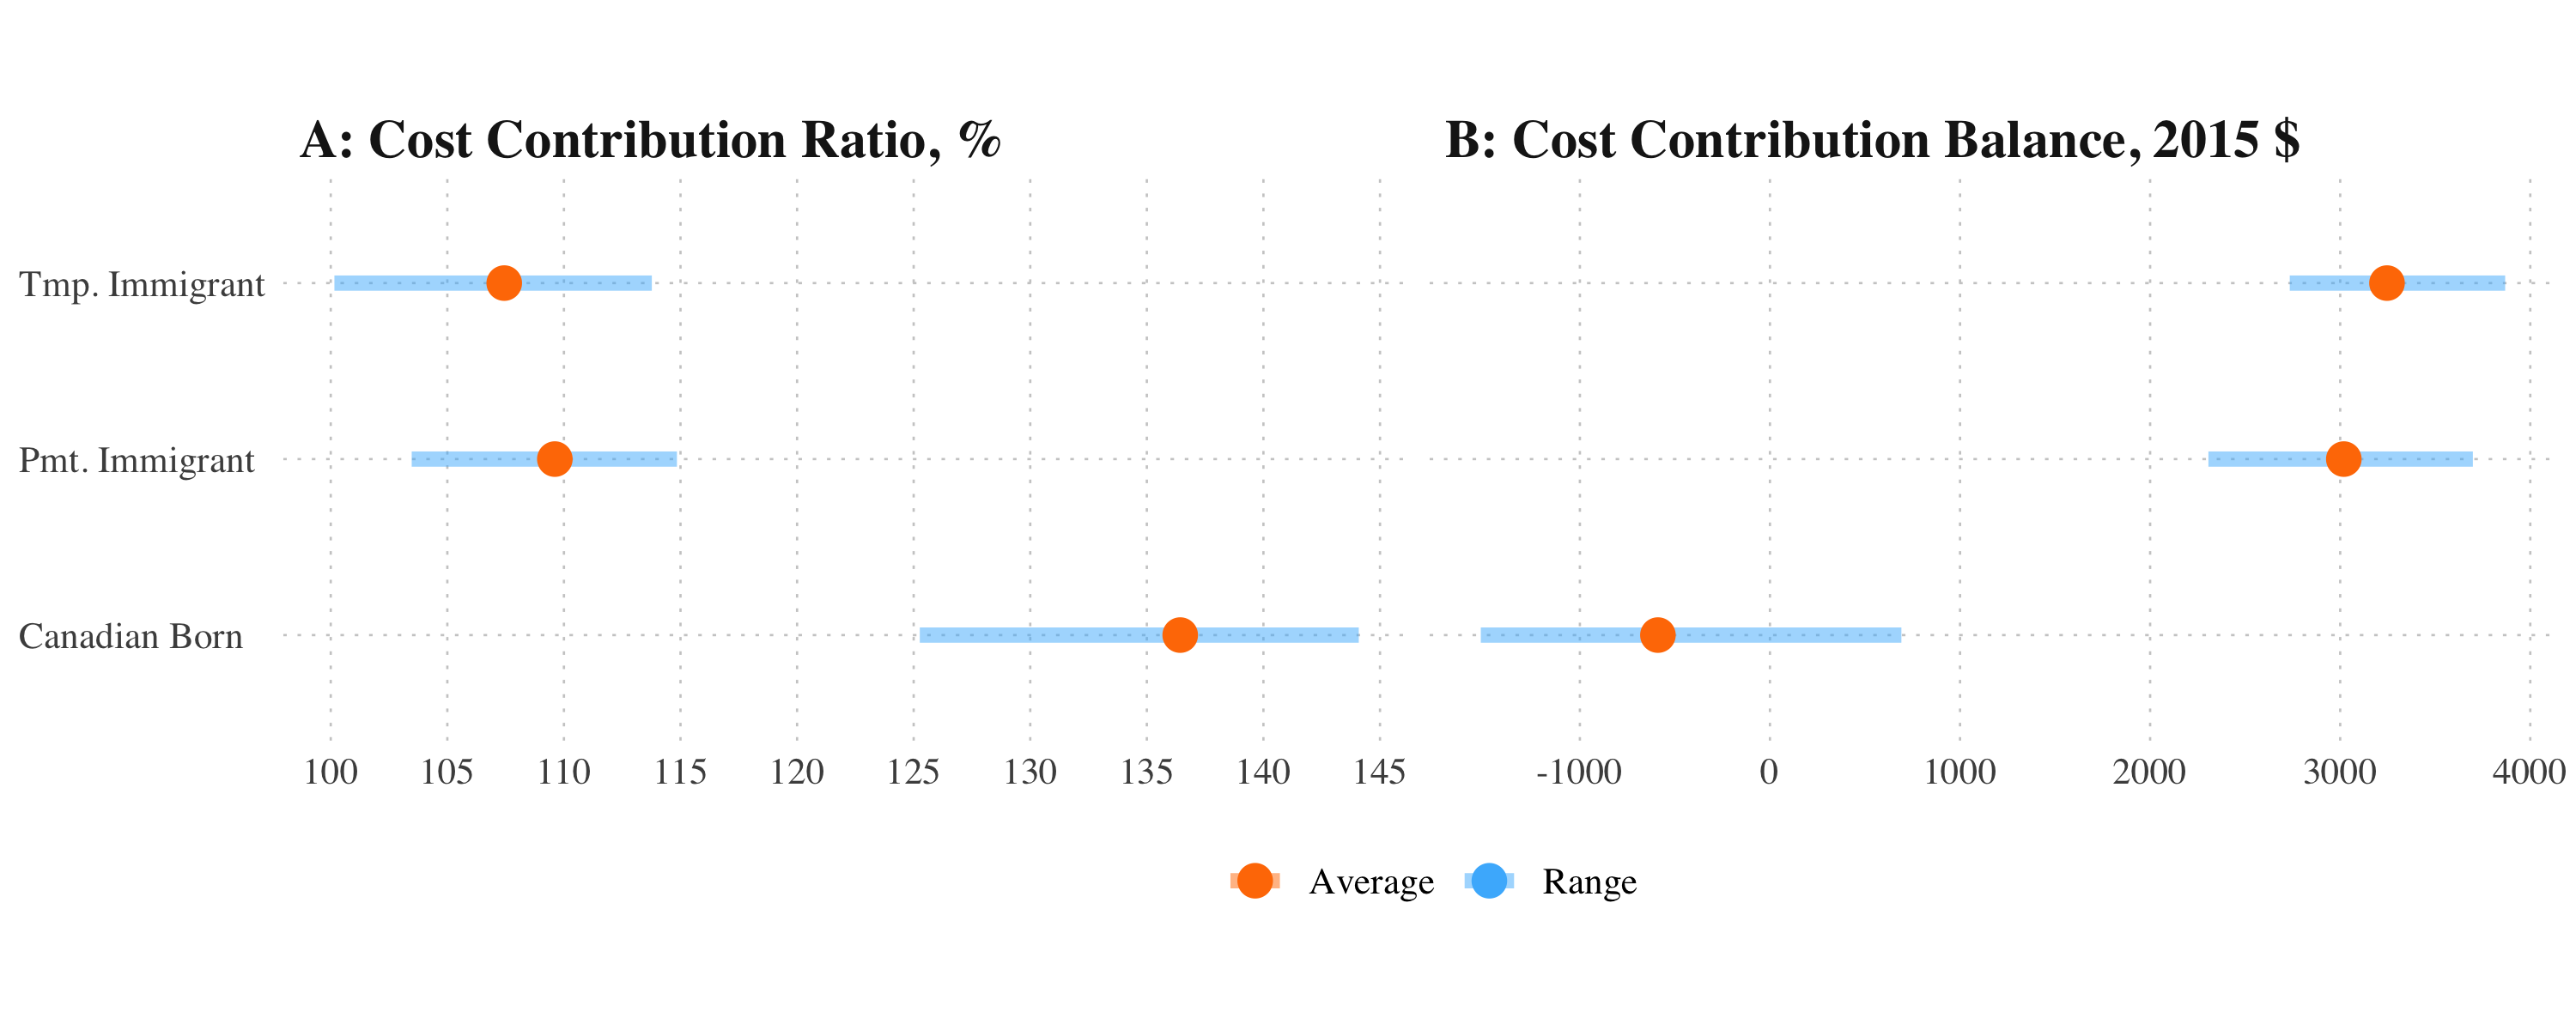
\includegraphics[width=1\textwidth]{./res/txSumAj.png}%
    \label{fig:txSumAj}%
\end{figure}%



  \begin{figure}[H]%
    \caption{Age Ajusted Cost Contribution Trends by Immigration Status between 1997 and 2015}
    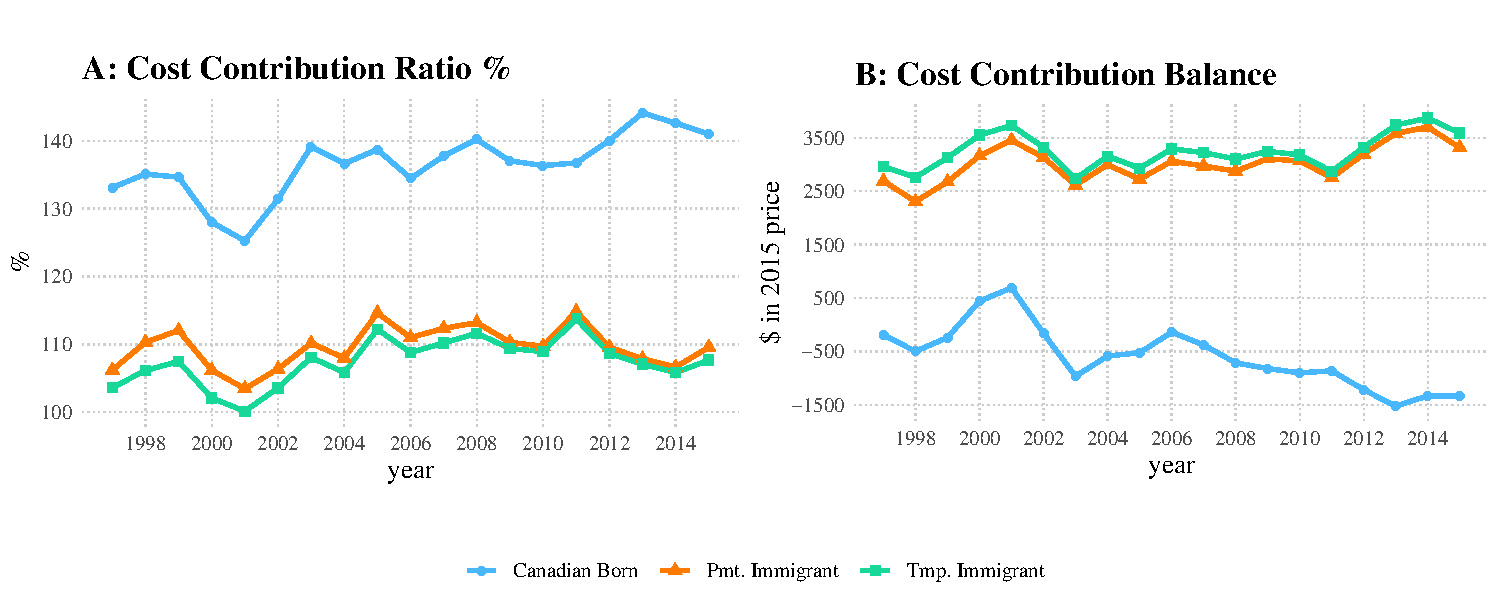
\includegraphics[width=1\textwidth]{./res/txTrendAj.pdf}%
    \label{fig:txTrendAj}%
\end{figure}%




    \begin{figure}[H]%
      \caption{Decomposition of per capita net transfer into demographic and transfer components for 1997 and 2015}
      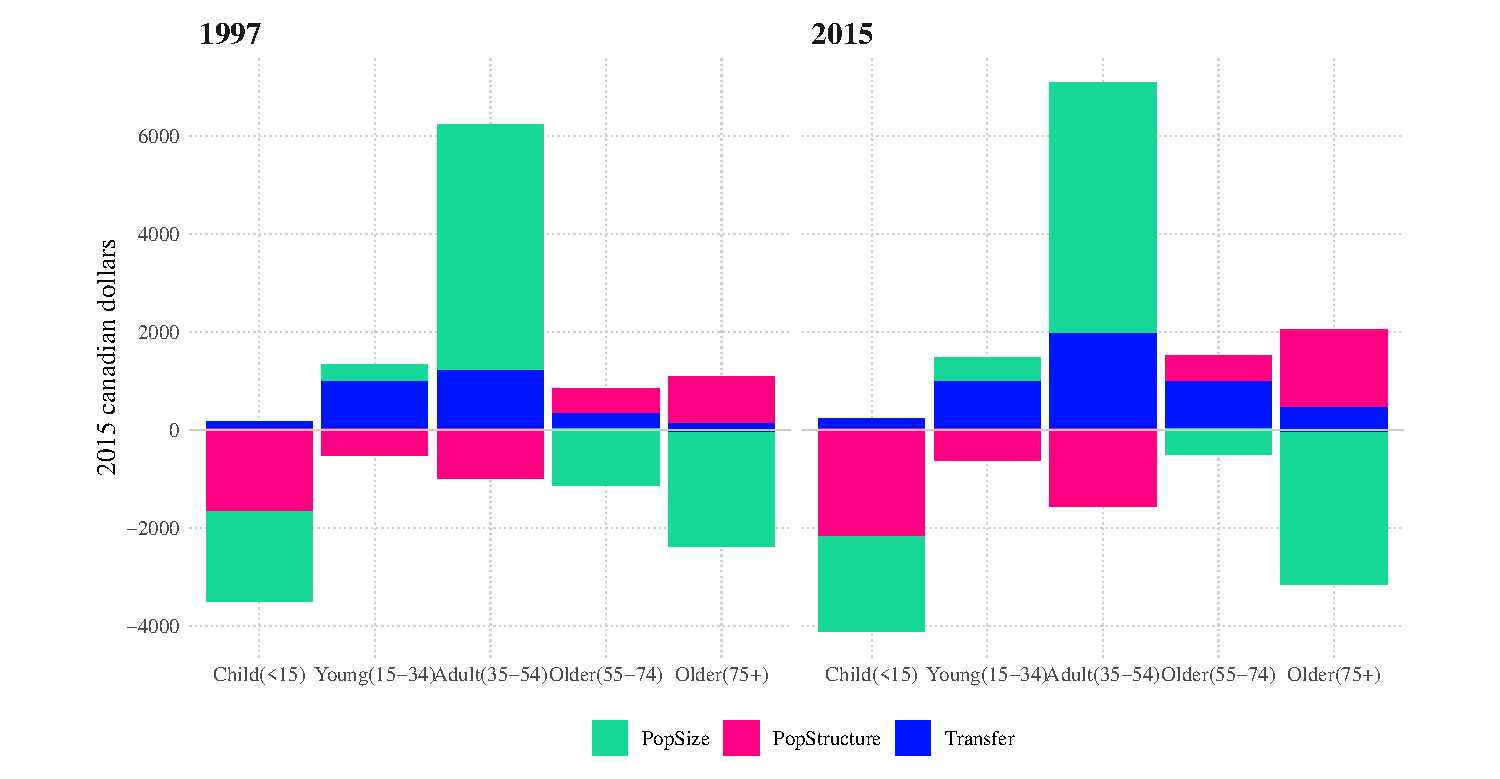
\includegraphics[width=1\textwidth]{./res/txb17_15.pdf}%
      \label{fig:txb17_15}%
  \end{figure}%



      \begin{figure}[H]%
        \caption{Immigrant to Native Difference for Components of Cost and Contribution between 1997 and 2015, sorted by decreasing weight}
        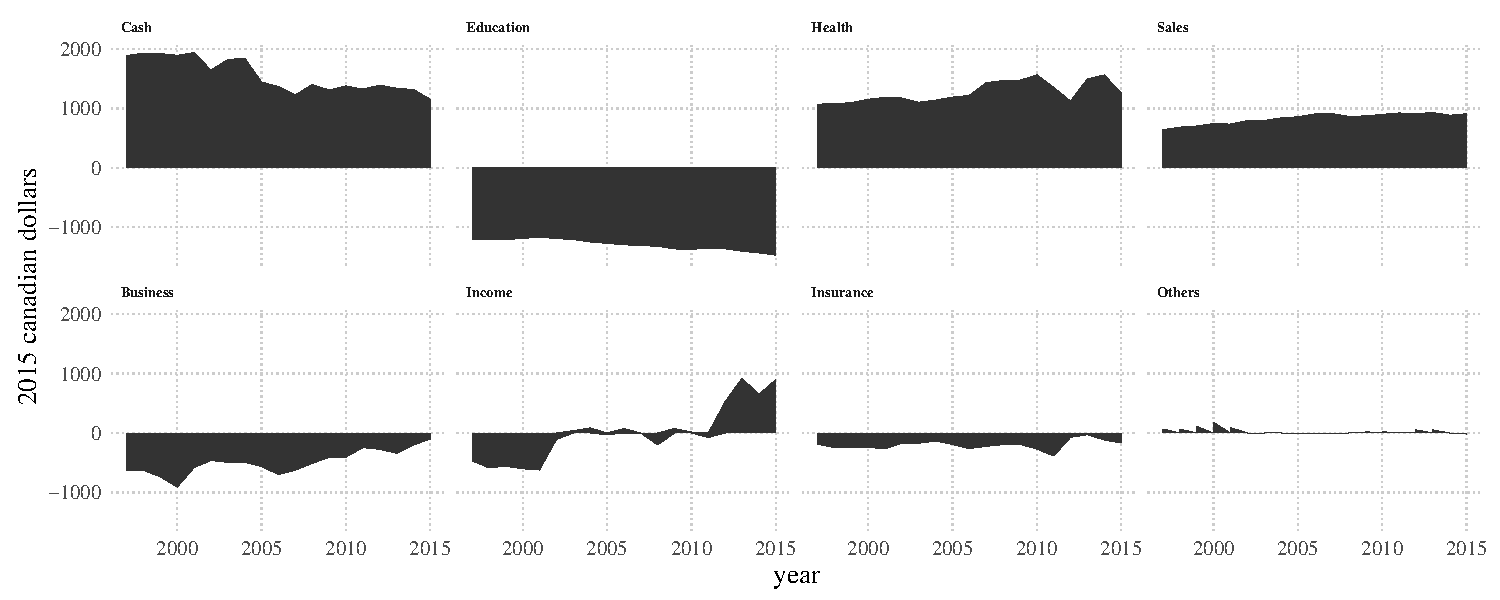
\includegraphics[width=1\textwidth]{./res/wgtComp.pdf}%
        \label{fig:wgtComp}%
    \end{figure}%
